\documentclass[10pt,final,a4paper,oneside,onecolumn]{article}

%%==========================================================================
%% Packages
%%==========================================================================
\usepackage[a4paper,left=3.5cm,right=3.5cm,top=3cm,bottom=3cm]{geometry} %% change page layout; remove for IEEE paper format
\usepackage[T1]{fontenc}                        %% output font encoding for international characters (e.g., accented)
\usepackage[cmex10]{amsmath}                    %% math typesetting; consider using the [cmex10] option
\usepackage{amssymb}                            %% special (symbol) fonts for math typesetting
\usepackage{amsthm}                             %% theorem styles
\usepackage{dsfont}                             %% double stroke roman fonts: the real numbers R: $\mathds{R}$
\usepackage{mathrsfs}                           %% formal script fonts: the Laplace transform L: $\mathscr{L}$
\usepackage[pdftex]{graphicx}                   %% graphics control; use dvips for TeXify; use pdftex for PDFTeXify
\usepackage{array}                              %% array functionality (array, tabular)
\usepackage{upgreek}                            %% upright Greek letters; add the prefix 'up', e.g. \upphi
\usepackage{stfloats}                           %% improved handling of floats
\usepackage{multirow}                           %% cells spanning multiple rows in tables
%\usepackage{subfigure}                         %% subfigures and corresponding captions (for use with IEEEconf.cls)
\usepackage{subfig}                             %% subfigures (IEEEtran.cls: set caption=false)
\usepackage{fancyhdr}                           %% page headers and footers
\usepackage[official,left]{eurosym}             %% the euro symbol; command: \euro
\usepackage{appendix}                           %% appendix layout
\usepackage{xspace}                             %% add space after macro depending on context
\usepackage{verbatim}                           %% provides the comment environment
\usepackage[dutch,USenglish]{babel}             %% language support
\usepackage{wrapfig}                            %% wrapping text around figures
\usepackage{longtable}                          %% tables spanning multiple pages
\usepackage{pgfplots}                           %% support for TikZ figures (Matlab/Python)
\pgfplotsset{compat=1.14}						%% Run in backwards compatibility mode
\usepackage[breaklinks=true,hidelinks,          %% implement hyperlinks (dvips yields minor problems with breaklinks;
bookmarksnumbered=true]{hyperref}   %% IEEEtran: set bookmarks=false)
%\usepackage[hyphenbreaks]{breakurl}            %% allow line breaks in URLs (don't use with PDFTeX)
\usepackage[final]{pdfpages}                    %% Include other pdfs
\usepackage[capitalize]{cleveref}				%% Referensing to figures, equations, etc.
\usepackage{units}								%% Appropriate behavior of units
\usepackage[utf8]{inputenc}   				 	%% utf8 support (required for biblatex)
\usepackage{csquotes}							%% Quoted texts are typeset according to rules of main language
\usepackage[style=ieee,doi=false,isbn=false,url=false,date=year,minbibnames=15,maxbibnames=15,backend=biber]{biblatex}
%\renewcommand*{\bibfont}{\footnotesize}		%% Use this for papers
\setlength{\biblabelsep}{\labelsep}
\bibliography{../../bib}

%%==========================================================================
%% Define reference stuff
%%==========================================================================
\crefname{figure}{Figure}{Figures}
\crefname{equation}{}{}

%%==========================================================================
%% Define header/title stuff
%%==========================================================================
\newcommand{\progressreportnumber}{28}
\renewcommand{\author}{Erwin de Gelder}
\renewcommand{\date}{March 12, 2020}
\renewcommand{\title}{Performance assessment of automated vehicles using real-world driving scenarios}

%%==========================================================================
%% Fancy headers and footers
%%==========================================================================
\pagestyle{fancy}                                       %% set page style
\fancyhf{}                                              %% clear all header & footer fields
\fancyhead[L]{Progress report \progressreportnumber}    %% define headers (LE: left field/even pages, etc.)
\fancyhead[R]{\author, \date}                           %% similar
\fancyfoot[C]{\thepage}                                 %% define footer


% Table stuff
\usepackage{booktabs}
\newcommand{\otoprule}{\midrule[\heavyrulewidth]}

\newcommand{\ud}{\,\mathrm{d}}
\newcommand{\expectation}[1]{\textup{E} \left[ #1 \right]}

\begin{document}
	
\begin{center}
	\begin{tabular}{c}
		\title \\ \\
		\textbf{\huge Progress report \progressreportnumber} \\ \\
		\author \\ 
		\date
	\end{tabular}
\end{center}

\section{Previous meeting minutes}

\begin{itemize}
	\item We discussed the planning regarding the publications and we agreed that I will not write another journal paper for quantifying the completeness of a data set and that I will go directly for a journal paper for the subject of test case generation. Furthermore, Bart suggested to mention the potential journal in which I want to publish.
	\item We discussed the paper titled ``Real-World Scenario Mining for the Assessment of Automated Vehicles''.
\end{itemize}

\section{Summary of work}

\begin{itemize}
	\item I submitted the paper titled ``Real-World Scenario Mining for the Assessment of Automated Vehicles'' to the International Transportation Systems Conference (ITSC).
	\item I received feedback on the manuscript of the ontology article. A major revision has been requested. Earlier this week, I submitted a revised version of the manuscript.
	\item In \cref{tab:journals}, I listed various interesting journals and their 2-year impact factor (IF) and scimago journal rank (SJR).
	\item I looked in several methods for improving the test case generation. For more information, see \cref{sec:test case generation}.
\end{itemize}

\begin{table}[b!]
	\centering
	\caption{Various journals related to my research and their 2-year impact factor (IF) and scimago journal rank (SJR) in 2018.}
	\label{tab:journals}
	\begin{tabular}{lrr}
		\toprule
		Journal name & IF & SJR \\ \otoprule
		Transportation Research Part B: Methodological	& 5.508	& 2.92 \\
		Transportation Research Part C: Emerging Technologies &	7.290 & 2.61 \\
		Transportation Research Part A: Policy and Practice &	4.430 &	2.04\\
		Transportation Research Part E: Logistics and Transportation Review &	5.245 &	1.97\\
		Transportation Research Part D: Transport and Environment &	4.752 &	1.45\\
		IEEE Transactions on Intelligent Transportation Systems &	7.420 &	1.41\\
		Journal of Intelligent Transportation Systems &	3.617 &	1.39\\
		Safety Science &	4.350 &	1.29\\
		IEEE Transactions on Vehicular Technology &	6.413 &	1.09\\
		IEEE Vehicular Technology Magazine &	5.571 &	1.05\\
		Transportation Research Part F: Traffic Psychology and Behaviour &	2.770 &	0.99\\
		Traffic Injury Prevention &	1.686 &	0.84\\
		IEEE Intelligent Transportation Systems Magazine &	4.227 &	0.57\\
		Transportation Research Record &	0.955 &	0.54\\
		IET Intelligent Transport Systems &	2.949 &	0.51\\
		International Journal of Intelligent Transportation Systems Research &	1.382 &	0.31\\
		IEEE Transactions on Intelligent Vehicles (since 2016) & N.A. & N.A. \\	
		Vehicles (really new)& N.A. & N.A. \\
		\bottomrule
	\end{tabular}
\end{table}
	


\section{Future plans}

In \cref{fig:planning}, the updated planning is shown. There are a few changes compared to the planning shown in the previous progress report:
\begin{itemize}
	\item A second journal article on the subject of ``completeness'' is not considered.
	\item There are no conference papers considered for the test case generation.
	\item I added potential journals in which I want to publish:
	\begin{itemize}
		\item For the overall methodology, my preferred choice would be the IEEE ITS Magazine. Although this journal has a relatively low SJR of 0.57 (see \cref{tab:journals}), I think it is suitable because this journal is generally less technical and I expect this paper to be less technical too.
		\item Because I expect that the article on test case generation to be relatively technical, I think IEEE Transactions on ITS is suitable. Transportation Research Part B and IEEE Transactions on IV are good alternatives.
		\item Similarly, I think the work on scenario risk quantification is suitable for three aforementioned journals. In \cref{fig:planning}, I mentioned IEEE Transactions on IV as the preferred journal, but this could as well be IEEE Transactions on ITS and Transportation Research Part B.
	\end{itemize}
\end{itemize}

\begin{figure}[t]
	\centering
	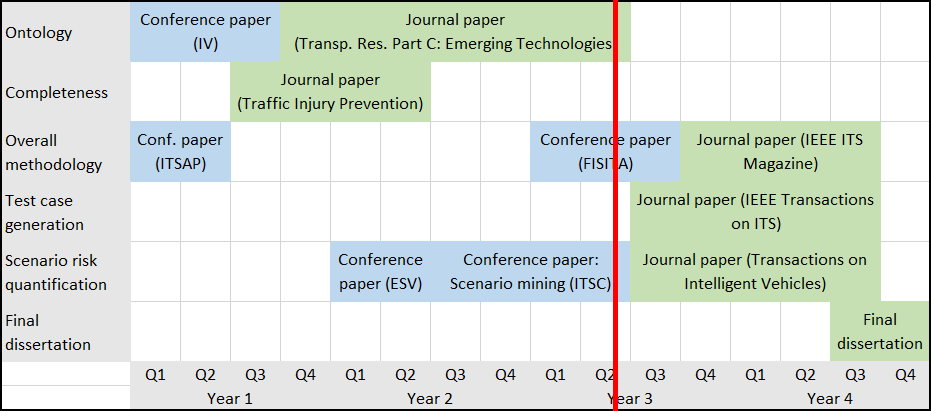
\includegraphics[width=\linewidth]{planning.png}
	\caption{Proposed planning at the time of this report. The red line indicated the time when writing this report.}
	\label{fig:planning}
\end{figure}

My plan on the near future is to focus on generating realistic test cases as described in \cref{sec:realistic}. This involves:
\begin{itemize}
	\item Perform a literature study to find different methods for defining a variable bandwidth.
	\item Try out the different methods for the variable bandwidth on some hypothetical data and some real data.
	\item Perform a literature study to find more information on ``evading the curse of dimensionality'' by assuming certain dependence structures as explained in \cref{sec:realistic}.
	\item Try out different methods to get better estimates of the pdf given a large number of parameters.
\end{itemize}

\section{Test case generation}
\label{sec:test case generation}

There are two interesting topics to look into:
\begin{enumerate}
	\item Generate \emph{realistic} test cases. 
	\item Emphasize test cases in which the system under test shows critical behavior.
\end{enumerate}

Both these topics might be addressed in a different article. I will describe shortly both topics. However, my focus will be on the first topic.


\subsection{Generate realistic test cases}
\label{sec:realistic}

To generate realistic test cases, we base the test cases on observed scenarios. To do this, we estimate the probability density function (pdf) of the parameters of a scenario and by drawing samples from this pdf, we generate test cases \autocite{deGelder2017assessment}. To be flexible with the shape of the underlying pdf, we use Kernel Density Estimation to estimate the pdf $f(\cdot)$:
\begin{equation} \label{eq:kde}
	\hat{f}(x) = \frac{1}{nh^d} \sum_{i=1}^n K\left( \frac{ \|x - X_i \| }{h} \right),
\end{equation}
where $X_i \in \mathds{R}^d, i\in\{1,\ldots,n\}$ represent the $d$-dimensional parameter vector of the $i$-th observed scenario, $h$ denotes the bandwidth, $K(\cdot)$ represents a kernel function, and $\|u\|$ denotes the euclidean distance of $u$. One way to improve \cref{eq:kde} is to consider a bandwidth that is not constant everywhere. This especially improves the estimation of the pdf near the tails of the distribution \autocite{sain1996locally,sain2002multivariate}. For example, we could consider a bandwidth that is different for each sample $X_i$; this is knows as a sample-point estimator:
\begin{equation}
	\hat{f}(x) = \frac{1}{n} \sum_{i=1}^n \frac{1}{h^d(X_i)} K\left( \frac{ \|x - X_i \| }{h(X_i)} \right).
\end{equation}

Choosing the bandwidth $h(X_i)$ is not a trivial task. I tried to use $k$-nearest neighbors (i.e., $h(X_i)$ equals the distance of $X_i$ toward its $k$-th closest neighboring point). When applying this to data from a Cauchy distribution --- which is an extreme case considering the heavy tails of this distribution --- the results are \emph{a lot} better. For future work, I want to search for different methods for calculating $h(X_i)$ and apply these methods on our data.

Another problem with $\cref{eq:kde}$ is the need for many data when more parameters are considered, i.e., when $d$ is large. With our current data, having 5 or more parameters ($d \geq 5$) is already problematic when applying \cref{eq:kde}. One way to improve this is to assume that not all parameters depend on all other parameters. To see this, consider, without loss of generality, that we can write $x$ as a combination of the parameter vectors $w\in\mathds{R}^{d_w}$, $y\in\mathds{R}^{d_y}$, and $z\in\mathds{R}^{d_z}$, $d_w+d_y+d_z=d$:
\begin{equation}
	x = \begin{bmatrix}
	w \\ y \\ z
	\end{bmatrix}.
\end{equation}
In this case, we can formulate the likelihood of $x$, $f(x)$ as follows:
\begin{equation}
	f(x) = f_{wyz}(w,y,z) = f_{wy}(w,y) \cdot \frac{f_{wyz}(w,y,z)}{f_{wy}(w,y)} = f_{wy}(w,y) \cdot f_{z|wy}(z | w, y),
\end{equation} 
where $f_{z|wy}(z|w,x)$ denotes the likelihood of $z$ given $w,y$. Now, let us assume that $f_{z|wy}(z|w,y) \approx f_{z|y}(z|y)$. In that case, we have
\begin{equation} \label{eq:approximation}
	f(x) \approx f_{wy}(w,y) \cdot f_{zy}(z|y) = f_{wy}(w,y) \cdot \frac{f_{yz}(y,z)}{f_y(y)}.
\end{equation}
Estimating $f(x)$ using the approximation of \cref{eq:approximation} gives
\begin{equation} \label{eq:pair}
	\hat{f}(x) = \hat{f}_{wy}(w,y) \cdot \frac{\hat{f}_{yz}(y,z)}{\hat{f}_y(y)}.
\end{equation}
Given that $\hat{f}_y(y) = \int_{\mathds{R}^{d_z}} \hat{f}_{yz}(y,z) \ud z$, we need to estimate two pdfs, but these two pdfs have a lower dimension than $\hat{f}(x)$. Hence, if the approximation in \cref{eq:approximation} is accurate, it is expected that \cref{eq:pair} gives a better estimate than \cref{eq:kde}.
In literature, the assumption in \cref{eq:approximation} is the underlying principle of what is called ``pair-copula constructions'' or ``vine copulas'' \autocite{aas2009paircopula, czado2010paircopula,  nagler2016evading}.



\subsection{Emphasize test cases with critical behavior}

Let $r(x)=\{0,1\}$ be the result of a simulation of a test case with parameters $x$. Suppose that $r(x)=1$ means that the system shows critical behavior. Naturally, we are interested in the expectation of $r(x)$, i.e., $\mu =\expectation{r(x)}$. A straightforward method to estimate $\mu$ is to use a Monte Carlo simulation:
\begin{equation}
	\hat{\mu} = \frac{1}{N} \sum_{i=1}^N r(x_i), \quad x_i \sim \hat{f}(x),
\end{equation}
where $N$ is the number of simulations and $x_i$ is the $i$-th parameter vector representing the $i$-th test case drawn from the estimated pdf $\hat{f}(\cdot)$.

In practice, $\mu$ is often close to zero. This means that a large number of simulations ($N$) is required to obtain a low relative variance of the estimated $\mu$ ($\textup{Var}[\hat{\mu}]/\mu$). This poses a problem, because simulations are costly. One way to speed up the estimation of $\mu$ is to draw samples from another distribution $\hat{h}(x)$ that puts more emphasize on the test cases that result in critical behavior. This is also known as importance sampling. The resulting simulations need to be weighted:
\begin{equation}
	\hat{\mu} = \frac{1}{N} \sum_{i=1}^N r(x_i) \frac{\hat{f}(x_i)}{\hat{h}(x_i)}, \quad x_i \sim \hat{h}(x),
\end{equation}
However, to choose $\hat{h}(x)$ is not trivial. Doing it incorrectly might result in a wrong estimate.

In \autocite{deGelder2017assessment}, we already proposed a method to determine $\hat{h}(x)$. The disadvantage of that method is that it involves a rather large number of initial simulations with test cases sampled from the original pdf $\hat{f}(x)$. A way to improve this is to first estimate a \emph{surrogate} model of the simulation and to use that \emph{surrogate} model to estimate a suitable $\hat{h}(x)$. In \autocite{dubourg2013metamodel}, this is done to reduce the number of required simulations (although the application is totally different).


\printbibliography

%\clearpage
%\includepdf[pages=-,pagecommand={},width=\paperwidth]{../../""/.pdf}

\end{document}